\newpage

\section{Właściwości}
Siarczek galu występuje w dwóch postaciach:
\begin{itemize}
	\item Siarczek galu(II) - $\mathbf{GaS}$
	\item Siarczek galu(III) - $\mathbf{Ga_{2}S_{3}}$
\end{itemize}

\subsection{Siarczek galu(II)}
$\mathbf{GaS}$ tworzy bezbarwne lub żółte kryształki układu heksagonalnego, grupa przestrzenna
$\mathbf{P\;6_{3}/mmc}$. Kryształ siarczku galu $\mathbf{(GaS)}$ należy do rodziny półprzewodników warstwowych III-VI. Krystalizuje się w sześciokątnej strukturze o parametrach sieci $a = 0,3578$ i $c = 1,547$ nm. Każda warstwa w strukturze krystalicznej składa się z dwóch atomów galu i dwóch atomów siarki ułożonych w stos wzdłuż osi $c$ z powtarzającą się jednostką $\mathbf{S-Ga-Ga-S}$.
\begin{figure}[H]
	\begin{center}
		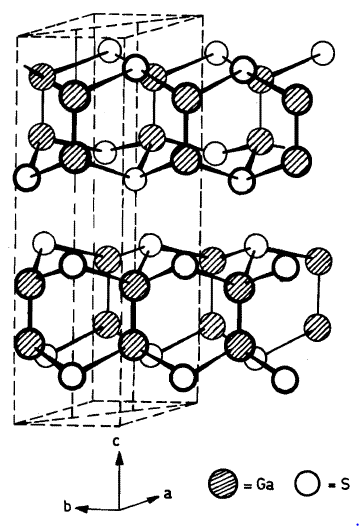
\includegraphics[width=0.5\linewidth]{Wlasciwosci/GaS_Schematic_Structure.png}
		\caption{Schematyczna reprezentacja struktury krystalicznej $\mathbf{GaS}$ [1]}
	\end{center}
\end{figure}
W kryształach $\mathbf{GaS}$ dominują słabe siły van der Waalsa w oddziaływaniach międzywarstwowych. Silne kowalencyjne siły dominują w oddziaływaniach wewnątrzwarstwowych.
$\mathbf{GaS}$ to półprzewodnik szerokopasmowy, który jest obiecującym materiałem. Skośna przerwa energetyczna wynosi $2.5eV$, a prosta wynosi $2.95eV$. Materiał umożliwia
wytwarzanie niebieskich urządzeń emitujących światło [1].

\newpage

\subsection{Siarczek galu(III)}
$\mathbf{Ga_{2}S_{3}}$ tworzy jasnożółte kryształki układu kubicznego, grupa przestrzenna
$\mathbf{F\;\overline{4}3m}$.
\begin{figure}[H]
	\begin{center}
		\begin{minipage}[h]{0.3\linewidth}
			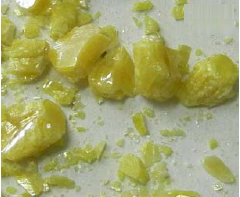
\includegraphics[width=1\linewidth]{Wlasciwosci/Ga2S3_View_Bridgman_Method.png}
		\end{minipage}
		\begin{minipage}[h]{0.3\linewidth}
			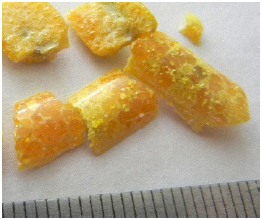
\includegraphics[width=1\linewidth]{Wlasciwosci/Ga2S3_View_Flux_Method.png}
		\end{minipage}
		\caption{Kryształki siarczku galu(III). Po lewej stronie $\mathbf{Ga_{2}S_{3}}$ wytworzony metodą Bridgmana. Po prawej $\mathbf{Ga_{2}S_{3}}$ wytworzony metodą flux-melt.[3]}
	\end{center}
\end{figure}
$\mathbf{Ga_{2}S_{3}}$ jest materiałem półprzewodnikowym o stosunkowo szerokiej (2.8eV) i prostej przerwie energetycznej. Ze względu na budowę warstwową jest rozważany jako perspektywiczny materiał do zastosowań w nanoelektronice i fotonice oraz do generacji sygnałów THz. Dodatkową jego zaletą jest silna anizotropia optyczna i jest rozważany jako materiał nieliniowy do generacji drugiej harmonicznej (SHG) w zakresie średniej podczerwieni.
\begin{figure}[H]
	\begin{center}
		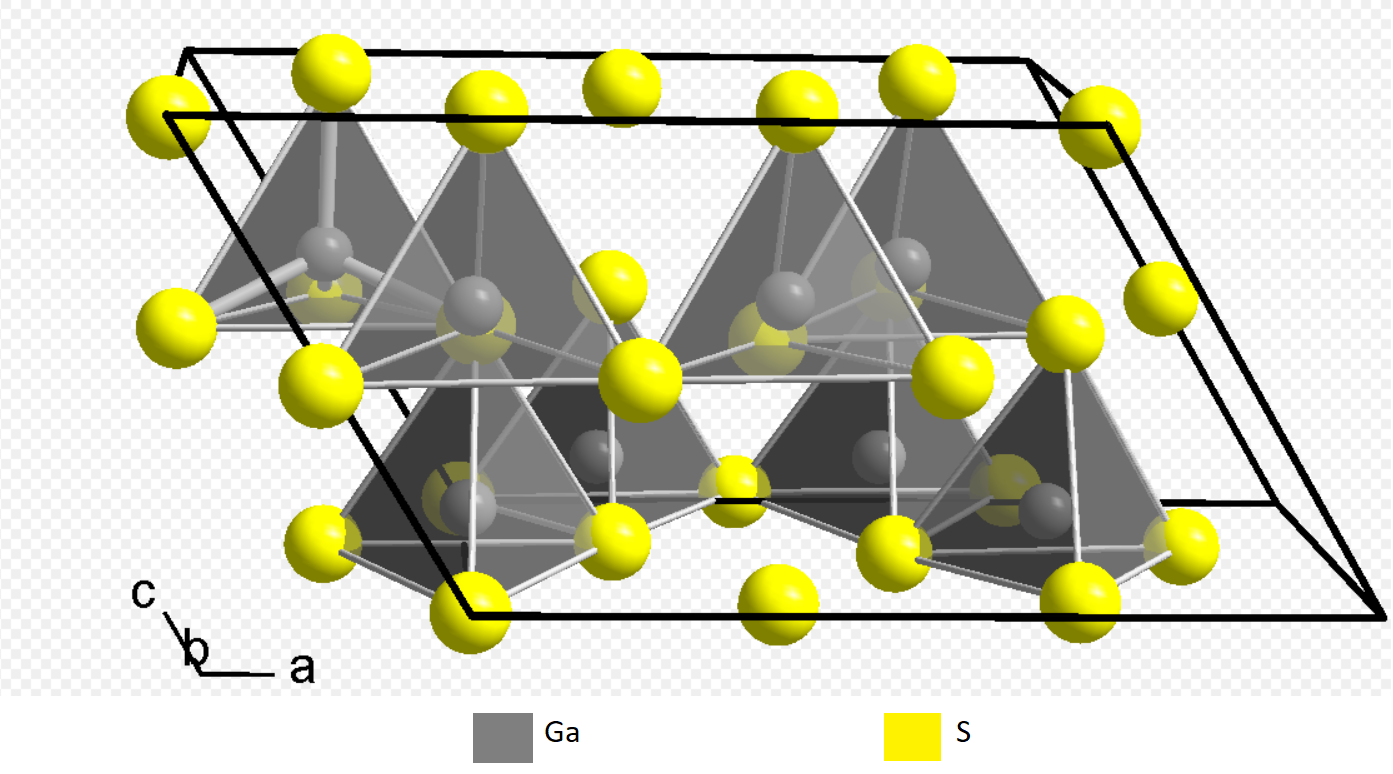
\includegraphics[width=0.6\linewidth]{Wlasciwosci/Ga2S3_Schematic_Structure2.png}
		\caption{Struktura krystaliczna $\mathbf{Ga_{2}S_{3}}$.[2]}
	\end{center}
\end{figure}



